\documentclass[../main-notes.tex]{subfiles}

\begin{document}

\section{Hyperbola}

A hyperbola is a curve defined by all points that satifies that the difference of the distance from a point $P$ to a point $F_1$ with the distance from a point $P$ to a point $F_2$ remains as a constant value of $2a$, as shown in figure\ref{fig-hyperbola}.
The distance between point $F_1$ and $F_2$ is defined to be $2c$.

\begin{marginfigure}
    \centering
    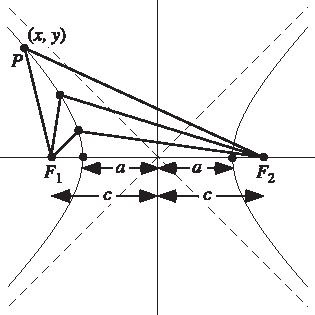
\includegraphics[width=\textwidth]{../Figures/hyperbola/HyperbolaFoci_750.pdf}
    \caption{Skecth of an hyperbola}\label{fig-hyperbola}
\end{marginfigure}

\subsection{Derivation of the equation}
We are going to call the distance from point $P$ to point $F_1$ as $r_1$, and the distance from point $P$ to point $F_2$ as $r_2$.
By definition, the substraction of those distances needs to be equal to $2a$, therefore we have the following equation,
\begin{gather*}
    \sqrt{\qty(x-c)^2+y^2} - \sqrt{\qty(x+c)^2+y^2} = 2a.
\end{gather*}
As before, we are going to modify that equation to express it in a more friendly way, taking into account that $b^2=c^2-a^2$,
\begin{align*}
    \left[\sqrt{\qty(x-c)^2+y^2}\right]^2 &= \left[2a - \sqrt{\qty(x+c)^2+y^2}\right]^2 \\
    \qty(x-c)^2+y^2 &= 4a^2 - 4a\sqrt{\qty(x+c)^2+y^2} + \qty(x+c)^2+y^2 \\
    \cancelto{0}{x^2} -2cx +\cancelto{0}{c^2} +\cancelto{0}{y^2} &= 4a^2 - 4a\sqrt{\qty(x+c)^2+y^2} + \cancelto{0}{x^2} + 2cx +\cancelto{0}{c^2} +\cancelto{0}{y^2} \\
    \frac{1}{4a}\left[4a\sqrt{\qty(x+c)^2+y^2}\right] &= \frac{1}{4a}\left[4a^2+4cx\right] \\
    \left[\sqrt{\qty(x+c)^2+y^2}\right]^2 &= \left[a+\frac{cx}{a}\right]^2 \\
    \qty(x+c)^2+y^2 &= a^2 + 2cx + \frac{c^2x^2}{a^2} \\
    x^2 + \cancelto{0}{2cx} + c^2 +y^2 &= a^2 + \cancelto{0}{2cx} + \frac{c^2x^2}{a^2} \\
    x^2 + c^2 +y^2 &= a^2 + \frac{c^2x^2}{a^2} \\
    x^2\cancelto{-b^2/a^2}{\qty(1-\frac{c^2}{a^2})} +y^2 &= \cancelto{-b^2}{a^2 - c^2} \\
    \frac{1}{-b^2}\left[\frac{-b^2}{a^2}x^2 +y^2\right] &= \cancelto{1}{\frac{-b^2}{-b^2}} \\
    \frac{x^2}{a^2} - \frac{y^2}{b^2} &= 1 \\
\end{align*}


\end{document}
